\documentclass[11pt,nocut]{article}

\usepackage{../latex_style/packages}
\usepackage{../latex_style/notations}

\title{\vspace{-2.0cm}%
	Optimization and Computational Linear Algebra for Data Science\\
Homework 12: Gradient descent}
\date{}
\author{Due on December 13, 2019}
\setcounter{section}{12}

\begin{document}
\maketitle
%\noindent\textbf{Rules:}
\centerline{\pgfornament[width=13cm]{89}}
{\small
	\begin{itemize}
		\item Unless otherwise stated, all answers must be mathematically justified.
		\item Partial answers will be graded. 
		\item You can work in groups but each student must write his/her own solution based on his/her own understanding of the problem. Please list on your submission the students you work with for the homework (his will note affect your grade).
		\item Late submissions will be graded with a penalty of $10\%$ per day late. Weekend days do not count: from Friday to Monday count $1$ day.
		\item Problems with a $(\star)$ are extra credit, they will not (directly) contribute to your score of this homework. However, for every $4$ extra credit questions successfully answered your lowest homework score get replaced by a perfect score.
		\item If you have any questions, feel free to contact myself (\texttt{leo.miolane@gmail.com}) or to stop at the office hours.
	\end{itemize}
}
\vspace{-0.4cm}
\centerline{\pgfornament[width=13cm]{89}}
\vspace{0.5cm}


\vspace{1mm}

\begin{problem}[2 points] The following plot shows the contour lines of a function $f:\R^2 \to \R$.
	\begin{figure}[H]
		\begin{center}
		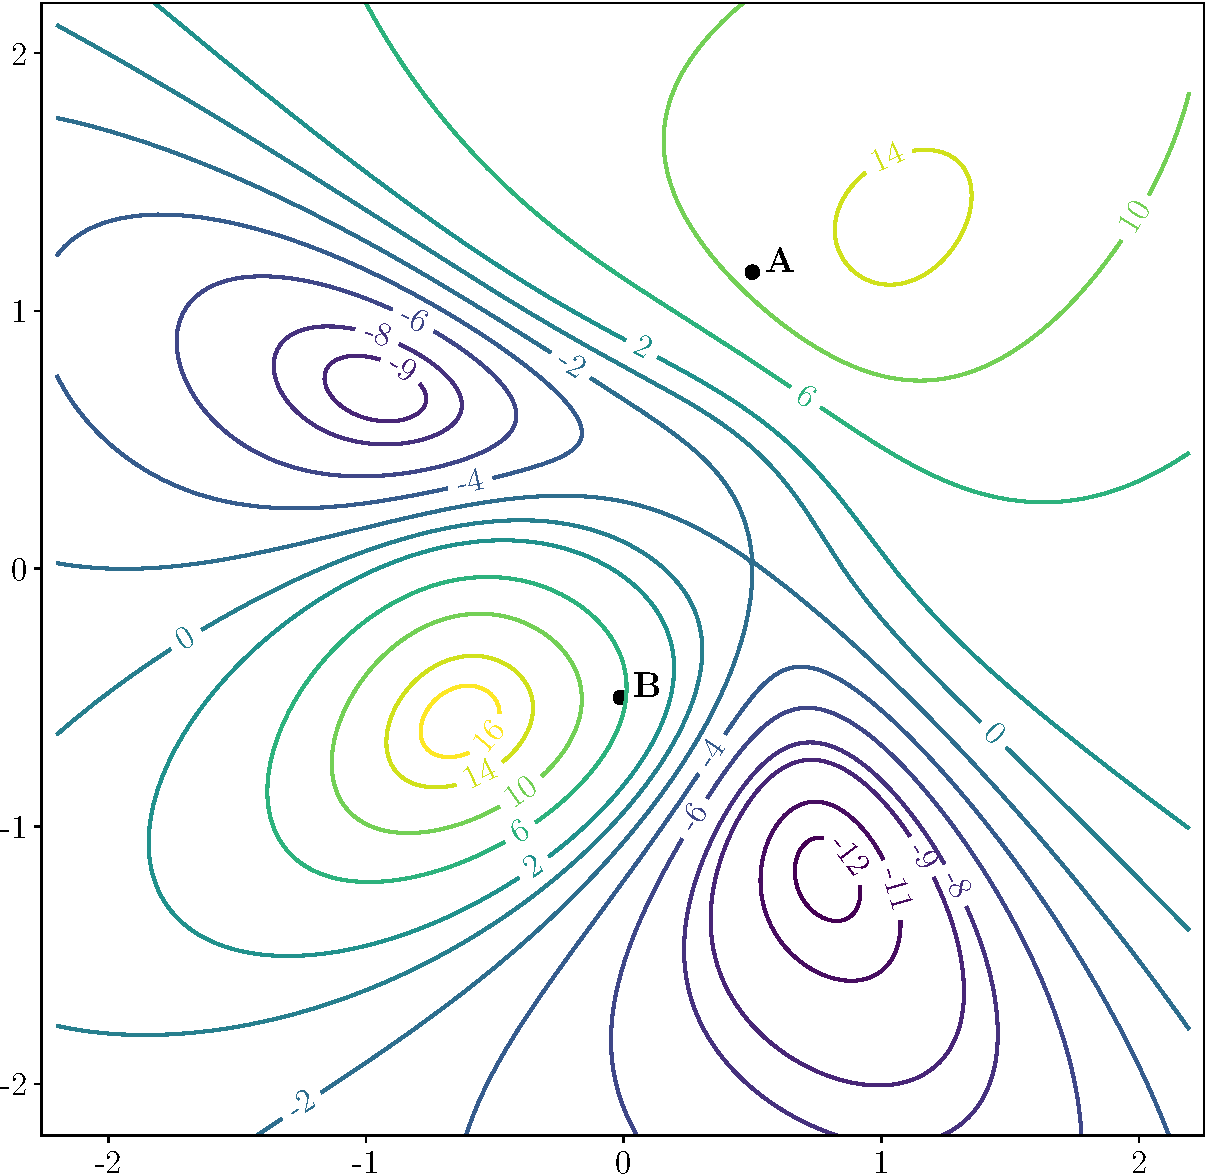
\includegraphics[width=11cm]{contours.pdf}
		\end{center}
	\end{figure}
	\begin{enumerate}[label=\normalfont(\textbf{\alph*})]
		\item Give (approximately) the coordinates of the global/local minimizers/maximizers, saddle points of $f$.
		\item Assume that we run gradient descent to minimize $f$. Will gradient descent converge to the global minimizer of $f$ when initialized at point $\bbf{A}$ ? at point $\bbf{B}$ ?
	\end{enumerate}
\end{problem}

\vspace{5mm}

\begin{problem}[5 points]\label{p:grad}
	Let $M \in \R^{d \times d}$ be a positive semidefinite matrix, $b \in \R^d$ and $c \in \R$. We aim at minimizing the quadratic function
	$$
	f(x) = \frac{1}{2} x^{\sT} M x - \langle x,b \rangle + c
	$$
	using gradient descent. 
	We assume that $M$ is positive definite (i.e.\ all its eigenvalues are positive).
	We let $\lambda_1 \geq \lambda_2 \geq \cdots \geq \lambda_d >0$ be its eigenvalues and let $v_1, \dots, v_d$ be an orthonormal basis of $\R^d$ consisting of associated eigenvectors ($Mv_i = \lambda_i v_i$ for all $i$).
	We write $L = \lambda_1$ and $\mu = \lambda_n$.
	\\

	We consider standard gradient descent with constant step-size $\beta$:
$$
x_{t+1} = x_t - \beta \nabla f(x_t).
$$
	\begin{enumerate}[label=\normalfont(\textbf{\alph*})]
		\item Show that $f$ is $L$-smooth, $\mu$-strongly convex and that $x^* = M^{-1} b$ is the unique minimizer of $f$.
		\item We now study the convergence of gradient descent to $x^*$. Show that for all $t \geq 0$,
			$$
			x_{t+1} - x^* = \big(\Id - \beta M \big)(x_t - x^*).
			$$
		\item From now, we set $\beta = 1/L$. Deduce from the previous question that for all $t \geq 0$
			$$
			\|x_t - x^* \| \leq \Big(1- \frac{\mu}{L}\Big)^{\! t} \, \|x_0 - x^*\|.
			$$
		\item We would like now to have something more precise than the error bound of the previous question. We define $w_t \defeq x_t -x^*$. Let 
			$$
			\alpha_1(t) = \langle v_1, w_t \rangle, \cdots, \alpha_d(t) = \langle v_d, w_t \rangle
			$$
			be the coordinates of $w_t$ in the orthonormal basis $(v_1, \dots, v_d)$.
			For $i \in \{1, \dots, d\}$, express $\alpha_i(t)$ in terms of $t,\lambda_i,L$ and $\alpha_i(0)$. 
		\item Using the previous question, justify the following sentence:
			\begin{center}
			\emph{
				<< Gradient descent converges towards the minimizer faster in directions given  by the eigenvectors of the Hessian of $f$ corresponding to large eigenvalues than in directions corresponding to eigenvectors with small eigenvalues.>>
			}
			\end{center}
		\item Show that for all $t \geq 0$
			$$
			\|x_t - x^* \| = \sqrt{\sum_{i=1}^d \Big(1-\frac{\lambda_i}{L}\Big)^{\!2t} \big\langle v_i, x_0-x^* \big\rangle^2}.
			$$
	\end{enumerate}
\end{problem}

\vspace{5mm}

\begin{problem}[3 points]
	In this problem, you will implement and compare gradient descent with or without momentum to minimize the Ridge cost function:
	$$
	f(x) = \frac{1}{2} \|Ax-y\|^2 + \frac{\lambda}{2} \|x\|^2.
	$$
	All the instructions and questions are in the Jupyter notebook \texttt{gradient\_descent.ipynb}.
	\\

	\textbf{It is intended that you code in Python and use the provided Jupyter Notebook. Please only submit a pdf version of your notebook (right-click $\to$ `print' $\to$ `Save as pdf').}
\end{problem}


\vspace{5mm}

\begin{problem}[$\star$]
	We take exactly the same setting of Problem~\ref{p:grad}, but we now consider gradient descent with momentum:
$$
x_{t+1} = x_t - \beta \nabla f(x_t) + \gamma(x_t -x_{t-1}),
$$
for $t \geq 1$,
where we take
$$
\beta = \frac{4}{(\sqrt{L} + \sqrt{\gamma})^2}
\qquad \text{and} \qquad
\gamma = \left(\frac{\sqrt{L}-\sqrt{\mu}}{\sqrt{L}+\sqrt{\mu}}\right)^{\! 2}.
$$
Show now that the $\alpha_i(t) \defeq \langle v_i, x_t - x^* \rangle$ satisfy a second order linear recurrence relation (as a sequence indexed by $t$). Using this relation, show that for all $t \geq 0$
$$
|\alpha_i(t)| \leq C_i \left(\frac{\sqrt{L}-\sqrt{\mu}}{\sqrt{L} + \sqrt{\mu}}\right)^{\! t}
$$
where $C_i$ is a constant that does not depend on $t$, but that may depend on $x_0,x_1, \mu$ and $L$ (a precise expression of $C_i$ is not expected). Deduce that for all $t \geq 0$
$$
\|x_t - x^*\| \leq C \left(\frac{\sqrt{L}-\sqrt{\mu}}{\sqrt{L} + \sqrt{\mu}}\right)^{\! t}
$$
where $C$ is a constant that does not depend on $t$.
\end{problem}

%\begin{problem}[$\star$]
	%We take exactly the same setting of Problem~\ref{p:grad}, but we now consider a variant of gradient descent:
%$$
%x_{t+1} = x_t - \beta \big(\nabla f(x_t) + z_t\big)
%$$
%where the $z_1,z_2, \dots, z_t, \dots$ are i.i.d.\ standard Gaussian vectors (of dimension $d$) that account for some noise.
%This is a simplistic model to study stochastic gradient descent: indeed the gradient used by SGD on minibatches can be interpreted as noisy version of the full gradient $\nabla f$. This is why we model the behavior of SGD by adding noise to $\nabla f$.
%\\

%\end{problem}


\vspace{1cm}
\centerline{\pgfornament[width=7cm]{87}}

%\bibliographystyle{plain}
%\bibliography{./references.bib}
\end{document}
